% Перестроение поверхности в 3d.
\subsection{Методы перестроения поверхности в трехмерном случае}

\subsubsection{Архитектура неструктурированной поверхностной расчетной сетки}

Решение задачи перестроения поверхности будем рассматривать на неструктурированной поверхностной расчетной сетке с треугольными ячейками \cite{Meshcheryakov2023GeoEvo}.
Элементами расчетной сетки являются узлы ($N$), ребра ($e$) и треугольные ячейки ($f$).
Для удобства каждый элемент сетки связан со всеми своими инцидентными элементами: так связаны между собой инцидентные узлы и ребра, узлы и ячейки, ребра и ячейки (см. рис.~\ref{fig:text_1_remesh3_architecture}).
Множество инцидентных узлов рассматриваемого ребра или ячейки будем обозначать $\mathscr{N}$, множество инцидентных ребер рассматриваемого узла или ячейки будем обозначать $\mathscr{E}$, множество инцидентных ячеек рассматриваемого узла или ребра будем обозначать $\mathscr{F}$.

\begin{figure}[ht]
\centering
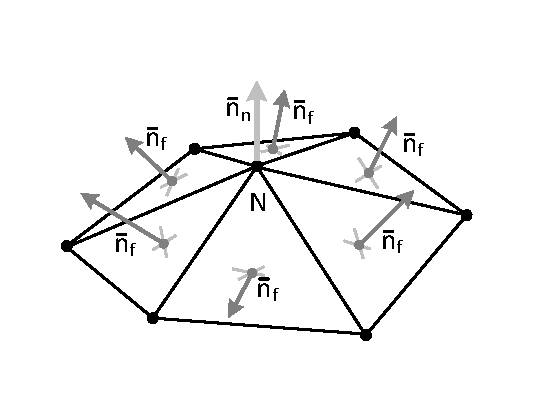
\includegraphics[width=0.5\textwidth]{pics/text_1_remesh_3d/pic_architecture.pdf}
\captionstyle{center}\caption{Архитектура расчетной сетки.}
\label{fig:text_1_remesh3_architecture}
\end{figure}

К расчетной сетке предъявляются следующие требования.
Во-первых, сетка должна быть целостной, то есть каждое ребро имеет ровно два инцидентных узла, отсутствуют изолированные и висячие узлы, а также изолированные ребра.
Во-вторых, все ячейки должны представлять собой треугольники (это гарантирует, что ячейка является плоской, так как четыре и более произвольных узлов могут не лежать в одной плоскости).
И в-третьих, рассматриваются только замкнутые сетки, представляющие собой поверхности, то есть каждое ребро имеет ровно две инцидентные ячейки (отсутствуют граничные ребра).
\begin{equation}\label{eqn:text_1_remesh3_arch}
\begin{cases}
\forall N \implies \mathscr{E}(N) > 2, \mathscr{F}(N) > 2, \\
\forall e \implies \mathscr{N}(e) = 2 , \mathscr{F}(e) = 2, \\
\forall f \implies \mathscr{N}(f) = 3 , \mathscr{E}(f) = 3. \\
\end{cases}
\end{equation}

\

В качестве дополнения также будем требовать, чтобы сетка представляла собой двустороннюю поверхность, для каждой ячейки однозначно определена нормаль к поверхности $\overline{n}_f$.
Также никакие два узла сетки не совпадают и отсутствуют ячейки с нулевой площадью (так как это сделает невозможным вычислений нормалей).
Для узла сетки будем рассматривать понятие нормали к поверхности и определять эту нормаль как
\begin{equation}
\overline{n}_n(N) = \frac{1}{|\mathscr{F}(N)|} \sum_{f \in \mathscr{F}(N)}{\overline{n}_f(f)}.
\end{equation}

%---------------------------------------------------------------------------------------------------

\subsubsection{Классические методы перестроения поверхности}

Центральная задача перестроения поверхности из-за накопления льда внутри ячеек расчетной сетки выглядит следующим образом.
Пусть известно, что в результате численного решения задачи ледообразования конечно-объемным методом \cite{Beaugendre2003Ice} в каждой ячейке сетки была вычислена масса накопленного льда ($m$).
Будем считать плотность льда постоянной, то есть в каждой ячейке также известен объем накопленного льда ($V$).
Для каждого узла сетки $N$ требуется найти его новое положение в пространстве $N'$, чтобы для каждой ячейки с узлами $ABC$ объем пространства, ограниченный фигурой $ABCA'B'C'$ соответствовал объему льда, накопленному в данной ячейке.

Следует отметить, что поставленная задача может не иметь точного решения, и в этом случае следует стремиться к минимизации ошибки по объему (когда фактически образовавшийся объем льда не слишком сильно отличается от целевого объема, то есть разница $V_{ABCA'B'C'} - V$ мала).

Задачу определения новых положений узлов расчетной сетки можно разделить на две задачи: определение направлений смещения узлов и определение величин смещения.

Простейшие классические методы перестроения выполняются в предположении, что направление смещения узла совпадает с нормалью, проведенной из этого узла.
Таким образом, необходимо лишь определить величину смещения.

\begin{figure}[h]
\centering
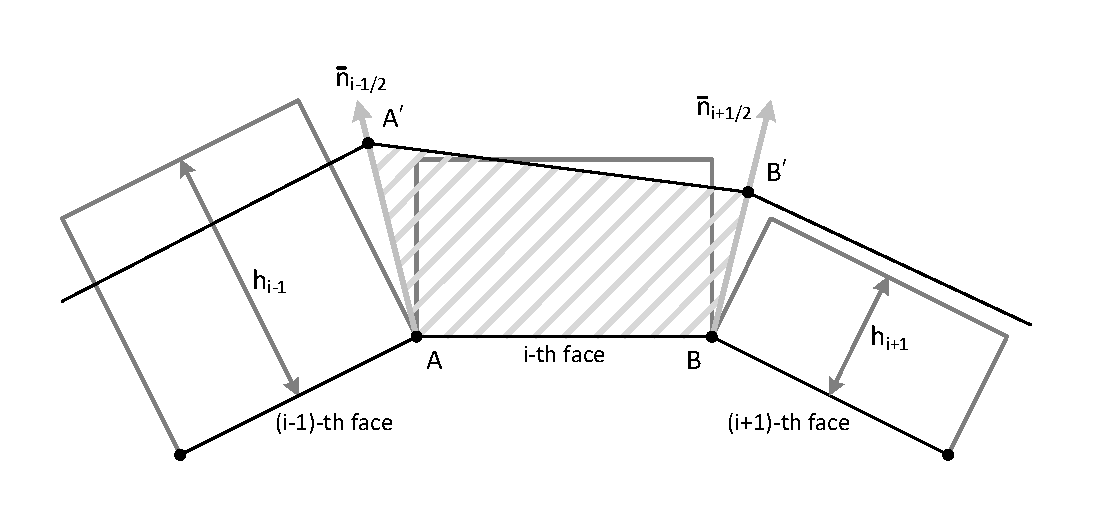
\includegraphics[width=0.8\textwidth]{pics/text_1_remesh_3d/pic_classical_methods_rectangles.pdf}
\caption{Перестроение поверхности с помощью метода прямоугольников в двумерном случае.}
\label{fig:text_1_remesh3_rect}
\end{figure}

\begin{figure}[ht]
\centering
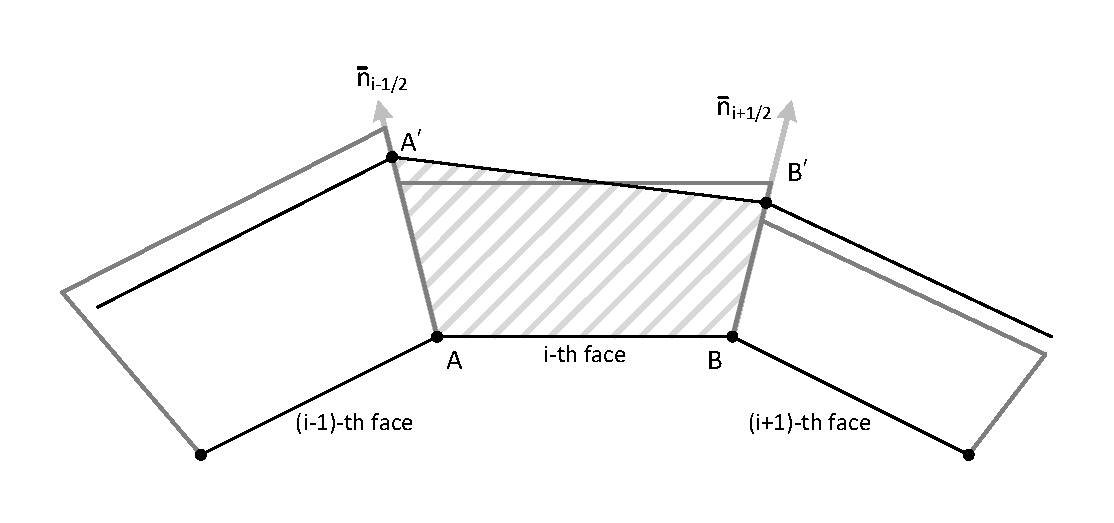
\includegraphics[width=0.8\textwidth]{pics/text_1_remesh_3d/pic_classical_methods_trapezoids.pdf}
\caption{Перестроение поверхности с помощью метода трапеций в двумерном случае.}
\label{fig:text_1_remesh3_trap}
\end{figure}

В качестве первого метода рассмотрим метод призм (в двумерной постановке аналогом данного метода является метод прямоугольников, продемонстрированный на рис.~\ref{fig:text_1_remesh3_rect}).
В этом методе входными данными является объем накопленного льда в каждой ячейке сетки ($V(f)$).
На первым шаге в каждой ячейке ищется толщина ледяного покрова в предположении, что лед в пределах одной ячейки имеет форму призмы, и ячейка является основанием этой призмы.
Тогда толщина ледяного покрова равняется $h(f) = \frac{V(f)}{S(f)}$, где $S(f)$ -- площадь ячейки.
После чего величина смещения каждого узла вычисляется просто как среднее арифметическое высот ледяного покрова во всех инцидентных ячейках:
\begin{equation}
h(N) = \frac{1}{|\mathscr{F}(N)|} \sum_{f \in \mathscr{F}(N)}{h(f)}.
\end{equation}

Второй метод можно назвать методом пирамид (в двумерной постановке аналогом данного метод является метод трапеций, показанный на рис.~\ref{fig:text_1_remesh3_trap}).
Входными данными также является объем накопленного льда в каждой ячейке сетки ($V(f)$).
Однако в отличие от предыдущего метода объем накопленного в ячейке льда представляется не призмой, а усеченной пирамидой, основанием которой является ячейка, а боковые ребра направлены вдоль нормалей узлов.
Высота этой усеченной пирамиды ищется из соотношения $V(f) = \frac{1}{3} h (2S + hS'_h + \sqrt{S(S + hS'_h)})$, где величина $S'_h$ определяется направлениями нормалей узлов ячейки.
Тогда как узлы ячейки являются точками первого основания построенной пирамиды, точки второго основания представляют собой новые положения узлов, вычисленные относительно рассматриваемой ячейки.
Таким образом, у каждого узла сетки вычисляется несколько новых положений (каждое из которых вычислено относительно своей инцидентной ячейки).
Для двумерного случая получается ровно два таких новых положения (так как в двумерном случае каждый узел имеет ровно две инцидентные ячейки), для трехмерного случае таких точек более двух.
Для выбора единственного нового положения узла сетки берется среднее значение из всех положений, вычисленных относительно инцидентных ячеек.

Из рассмотренных двух методов интуитивно создается впечатление, что метод пирамид должен быть более точным, так как он учитывает потери и избыток объема льда, образующиеся из-за изломов сетки (так как соседние ячейки не лежат в одной плоскости, то представление льда в ячейках в виде призм неизбежно приводит к образованию пробелов или наложений частей льда в виде призм друг на друга).

\begin{figure}[ht]
\centering
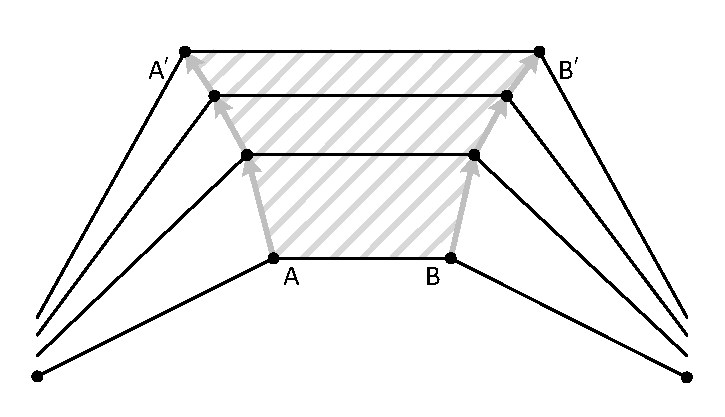
\includegraphics[width=0.6\textwidth]{pics/text_1_remesh_3d/pic_classical_methods_multilayer.pdf}
\captionstyle{center}\caption{Многослойное перестроение сетки.}
\label{fig:text_1_remesh3_multi}
\end{figure}

Вне зависимости от используемого метода перестроения значительно повысить точность можно с помощью многослойного подхода \cite{BourgaultCote2017}.
В этом случае вместо однократного перестроения сетки по объему накопленного льда в каждой ячейке ($V(f)$), выбирается фиксированное количество шагов перестроения $k$, а дальше процедура выполняется $k$ раз подряд, но с использованием объема накопленного в ячейке льда $\frac{V(f)}{k}$.
Точность повышается из-за того, что после каждого шага перестроения нормали в узлах сетки меняют свое направление, и общий объем наращиваемого льда становится более криволинейным, лучше учитывает геометрию сетки и, как следствие, точнее соответствует исходному значению $V(f)$ (см. рис.~\ref{fig:text_1_remesh3_multi}).

\subsubsection{Rebuilding with ice volume conservation}

The articles \cite{Thompson,Tong} describe a stable iterative mesh evolution algorithm that preserves the target volume of ice.
It uses several improvements over the classical methods.

The multilayer approach implemented in this method does not use a constant number of steps -- the value of the increased volume at each step of the algorithm is calculated based on the maximum allowable fraction of the icing time step, after exceeding which numerical instability may occur in the evolution of the surface.
The most obvious case occurs when the face normal projections intersect, in which case too large time step will cause the surface to fold.
In order to  identify faces that will exhibit such behavior at the
current time step, it is assumed that the volume formed by extruding
a triangular face using a parallel displacement plane forms a
prismatoid whose volume is given by the cubic function of the height
$h$:
\begin{equation}\label{Tong:1}
V(h)=ah+bh^2+ch^3.
\end{equation}
where the constants $a$, $b$, $c$ are determined by the  positions
of the face nodes, their normals, and the face normal.
Consider the roots of the quadratic equation, which is obtained as a result of differentiation of the equation (\ref{Tong:1}).
If the roots are positive real values, the smallest positive root determines the height at which the maximum volume is reached, which is denoted as $V_{max}$, otherwise the function is monotonic with increasing and no step restriction is required in this face.
From this, it is possible to calculate the maximum fraction of the icing time step that is required to ensure reasonable volume accumulation behavior.
In addition to this step size limit, a $\alpha_{jiao}$ stability limit has been introduced.
This stability limit is based on how normal directions change as the surface evolves \cite{Jiao}.
Then, the allowable fraction of the time step for the $i$th face is
defined as
\begin{equation*}
\alpha_{\Delta t}^i=
\begin{cases}
\min(s_{\Delta t}\frac{V_{\max}^i}{V_f},\alpha_{jiao},1), \text{if $V_{\max}^i$ exists}, \\
\alpha_{jiao}, \text{if $V_{\max}^i$ doesn't exist},
\end{cases}
\end{equation*}
where $s_{\Delta t}$ ($0 < s_{\Delta t} < 1$) is an  empirically
determined coefficient, $V_f$ is the current remaining ice increment
volume for the $i$th face.
Then, the volume built up for the current step is $\alpha_{\Delta t}
V_f$, where $\alpha_{\Delta t}$ is the global minimum value for all
faces.

Another important feature of the algorithm is the introduction of primary and null spaces, described in \cite{Jiao_null_space_smooth}.
If the evolutionary movement of mesh nodes occurs in primary space, then their movement in zero space will preserve the potential accuracy of the second order of the surface triangulation, so that we can maintain volume when smoothing the mesh surface.
The algorithm uses several types of smoothing.

The first smoothing is the smoothing of the normals in the mesh nodes and faces.
To make smoothing possible in zero space, all normals at nodes are calculated so that they lie in primary space, and the movement of nodes during ice buildup occurs only along their normals.
As evolution progresses, surface noise can increase, and if left unchecked, we can encounter a situation where the dihedral angle between the faces becomes too small and limits the maximum fraction of the icing time step.
To reduce surface noise, local smoothing is applied before ice builds up, adjusting the direction of node displacement in problem areas so that it more closely matches the directions of its neighbors.
This method can improve surface smoothness in some situations.
The main purpose of normal smoothing is to push points out of concave areas where normals can converge locally.
Normal smoothing is achieved using a series of weighted averages,
which are designed to give weight to the normals generated by
problem areas.

\begin{figure}[h]
\centering
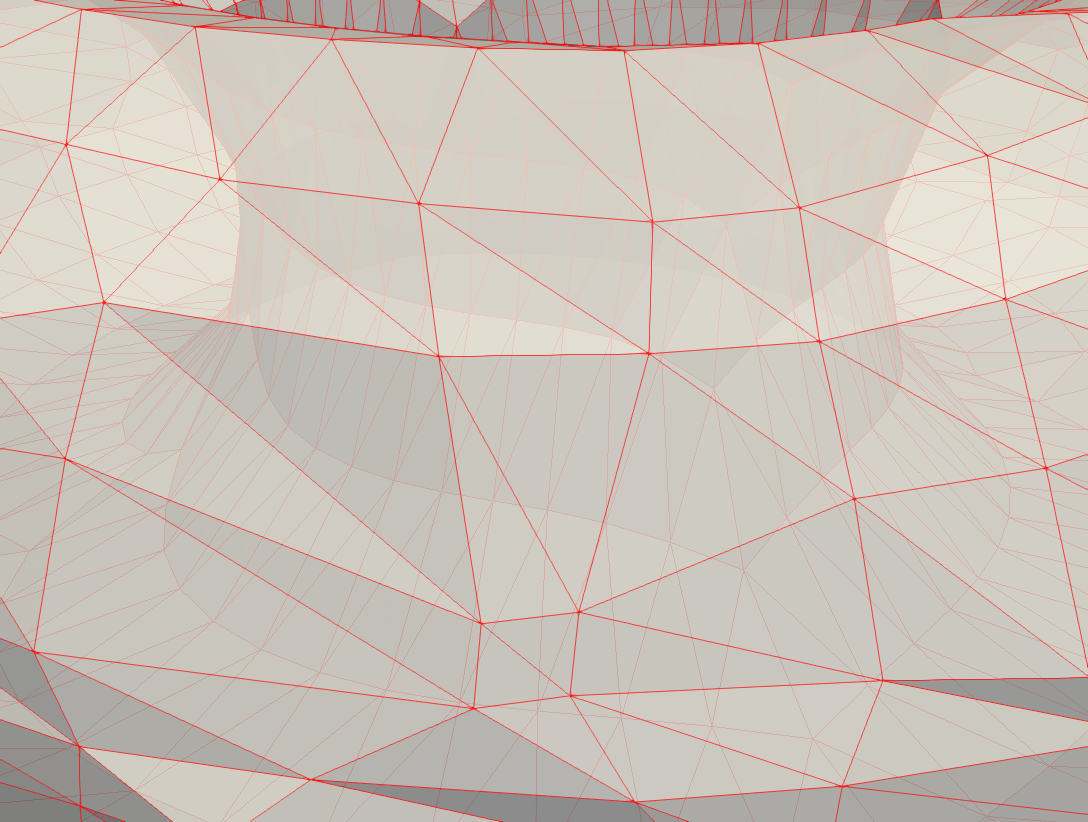
\includegraphics[width=\textwidth]{pics/text_1_remesh_3d/pic_smooth_before.png}
\caption{Mesh before null-space smoothing}\label{fig:pic_smooth_before}
\end{figure}

\begin{figure}[ht]
\centering
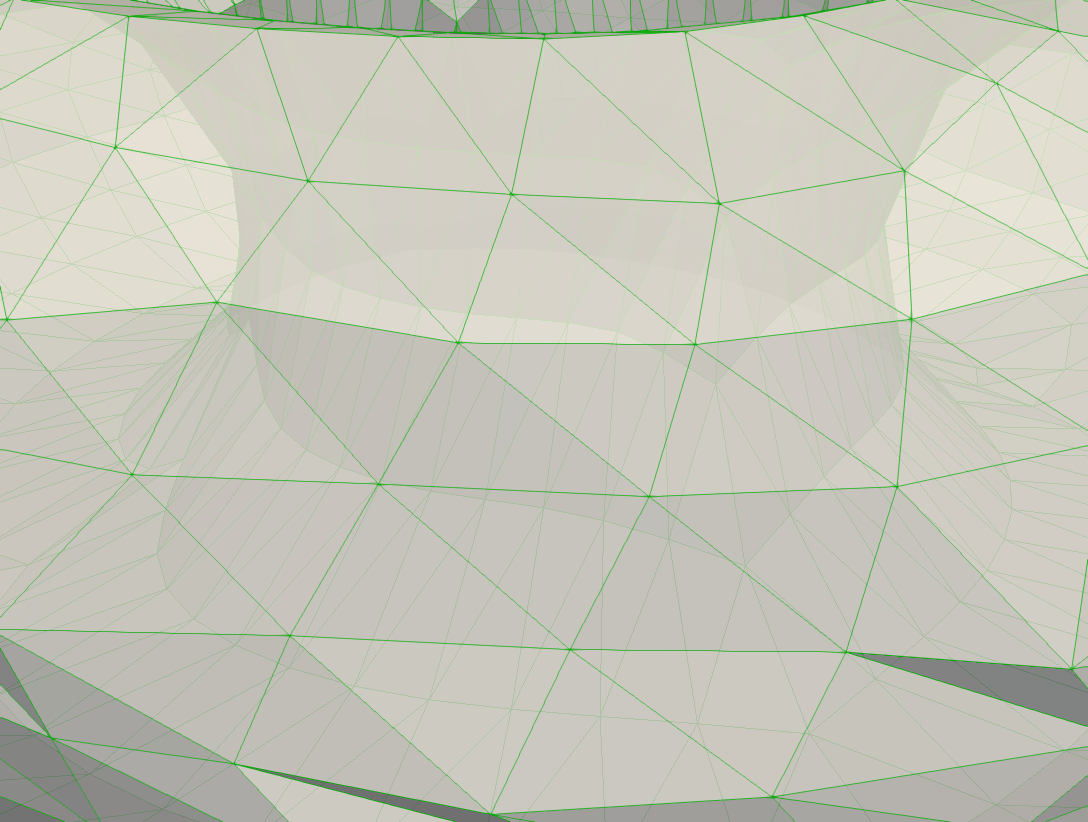
\includegraphics[width=\textwidth]{pics/text_1_remesh_3d/pic_smooth_after.png}
\caption{Mesh after null-space smoothing.}\label{fig:pic_smooth_after}
\end{figure}

The second smoothing is height smoothing.
After calculating the fraction of the time step and the volume that is increased for the current step, it is necessary to determine the height field for the evolution of the surface, which will correspond to this volume, in order to determine the offsets of the mesh nodes from it.
The solution $V(h_i) = \alpha_{\Delta t} V_f$ provides the initial height field that is used to move the surface.
The purpose of the additional height smoothing step is to filter out high-frequency noise in the height field by reducing the difference in height between adjacent faces.
Usually, the heights of two triangular faces that share a common edge will not be equal.
At this step, smoothing of heights is used while preserving the volume by redistributing it between adjacent faces.

The last type of smoothing is null-space smoothing.
Surface evolution will tend to pack nodes into concave regions where surface normals converge, while mesh expansion occurs in convex regions where surface normals diverge.
If the nodes are not reallocated, it may become impossible to continue with a productive and stable time step.
To improve the quality of the surface mesh, the nodes are redistributed on the surface using null-space smoothing.
This method is able to redistribute points while maintaining the integrity of the base geometry.
Null-space is defined by a tangent plane (for smooth areas),  a
tangent line (for surface wrinkles), or empty space (for corners),
nodes moving in it remain on the surface, so that the volume and
shape of the surface can be preserved
(Figs.~\ref{fig:pic_smooth_before} and \ref{fig:pic_smooth_after}).
